\section{Results \& Discussion}\label{s:results}


\subsection{Kinetic Sorption Model}



\begin{figure}[htb!]
  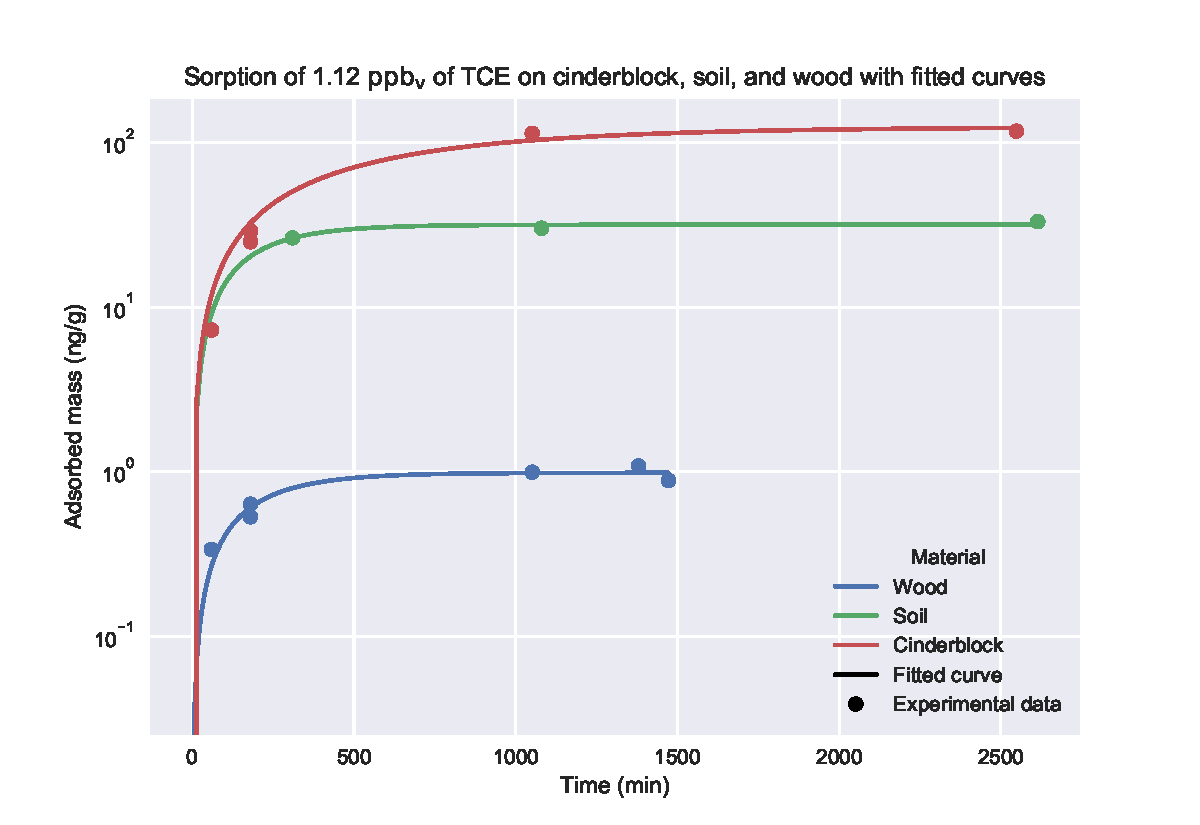
\includegraphics[width=\textwidth]{sorption_fit.pdf}
  \caption{}
  \label{fig:sorption_fit}
\end{figure}


\begin{table}[htb!]
  \caption{Fitted kinetic sorption parameters based on sorption experiment data.}
  \label{tbl:sorption_fit}
  \centering
  \begin{tabular}{l c c c}
    \toprule
    Material & $k_1 \; \mathrm{(1/hr)}$ & $k_2 \; \mathrm{(1/hr)}$ & $K$ \\
    \hline
    Wood & 0.32 & 44.90 & $7.10 \cdot 10^{-3}$ \\
    Drywall & 0.41 & 87.94 & $4.65 \cdot 10^{-3}$ \\
    Carpet & 0.26 & 58.74 & $4.42 \cdot 10^{-3}$ \\
    Paper & 0.04 & 88.37 & $4.55 \cdot 10^{-4}$ \\
    Soil & 0.34 & 2636.57 & $1.30 \cdot 10^{-4}$ \\
    Cinderblock & 0.10 & 4175.16 & $2.40 \cdot 10^{-5}$ \\
    \bottomrule
  \end{tabular}
\end{table}
